% ===== 第三章 问题二：盘入终止（碰撞）时刻（约3页） =====
\section*{三、问题二：盘入终止（碰撞）时刻判定}

\subsection{模型：双判据碰撞检测}
盘入过程中，龙头持续向内收拢，整条链逐渐拥挤。定义一个把手区域“失效/碰撞”事件，采用双判据并取先发生者：
\begin{enumerate}
\item \textbf{尾把手越过中心}：当 $s_{\rm head}(t)\le D_{223}$ 时，龙尾后把手弧长参数非正，物理上意味着整条 369.16m 的链已无法再向内盘入（尾部越过螺线中心）；[C6, Q2]
\item \textbf{非相邻板段相交}：把相邻把手中心的连线视为刚性板凳板段，若任意两个非相邻的板段（其把手下标差 $\ge2$）几何相交，则发生板凳碰撞。[C6,U2]
\end{enumerate}
终止时刻定义为
\begin{equation}\label{eq:tstar}
t^{\ast}=\min\Big\{t:\ s_{\rm head}(t)\le D_{223}\ \text{或}\ \exists\ \text{非相邻板段相交}\Big\}.
\end{equation}

\subsection{求解方法}
采用二分法在区间 $[0,\ S_0-D_{223}]$ 上求解 $t^{\ast}$，共 70 次迭代（相对容差 $\sim10^{-15}$）。板段相交判定采用标准线段相交双线性测试（容差 $10^{-9}$）。[log:q2.config]

\subsection{结果}
求得终止时刻 [log:q2.t\_star]
\begin{equation}\label{eq:tstar_val}
t^{\ast}=73.4303\ \text{s}.
\end{equation}
在该时刻，$s_{\rm head}(t^{\ast})=S_0-t^{\ast}=369.16$m $=D_{223}$，即触发判据为“尾把手到达中心”（严格取等之前，非相邻板段尚未相交；本文取判据 1 先发生）。[log:q2.collide\_event] 此刻龙头的位姿与速度、龙尾后把手的状态见表 \ref{tab:q2}，终止时刻整队位形见图 \ref{fig:q2}。

\begin{table}[H]\centering
\caption{问题二终止时刻 $t^{\ast}=73.4303$s 龙头/龙尾状态[log:q2]}
\label{tab:q2}
\begin{tabular}{lccc}
\toprule
把手 & $x$ (m) & $y$ (m) & $v$ (m/s) \\
\midrule
龙头前把手 & $-6.133685$ & $-5.192605$ & 1.000000 \\
龙尾后把手 & $0.000000$ & $0.000000$ & 0.990000 \\
\bottomrule
\end{tabular}
\end{table}

$result2.xlsx$ 写入终止时刻整队 224 个把手的位置与速度；表 \ref{tab:q2s} 给出指定节点（龙头前、第 1/51/101/151/201 节前、龙尾后）的完整位置速度。[log:q2.paper\_table\_sections, D4]

\begin{table}[H]\centering\small
\caption{问题二终止时刻指定节点位置与速度[log:q2.paper\_table\_sections]}
\label{tab:q2s}
\begin{tabular}{lcrr}
\toprule
节点 & 把手下标 & $x$ (m) & $y$ (m) \\
\midrule
第 1 节前 & 1 & $-7.530993$ & $-2.714536$ \\
第 51 节前 & 51 & 2.610444 & $-6.544296$ \\
第 101 节前 & 101 & 1.375347 & $-5.771365$ \\
第 151 节前 & 151 & $-0.965854$ & 4.452647 \\
第 201 节前 & 201 & $-2.268607$ & $-1.083333$ \\
\bottomrule
\end{tabular}
\end{table}

\begin{figure}[H]\centering
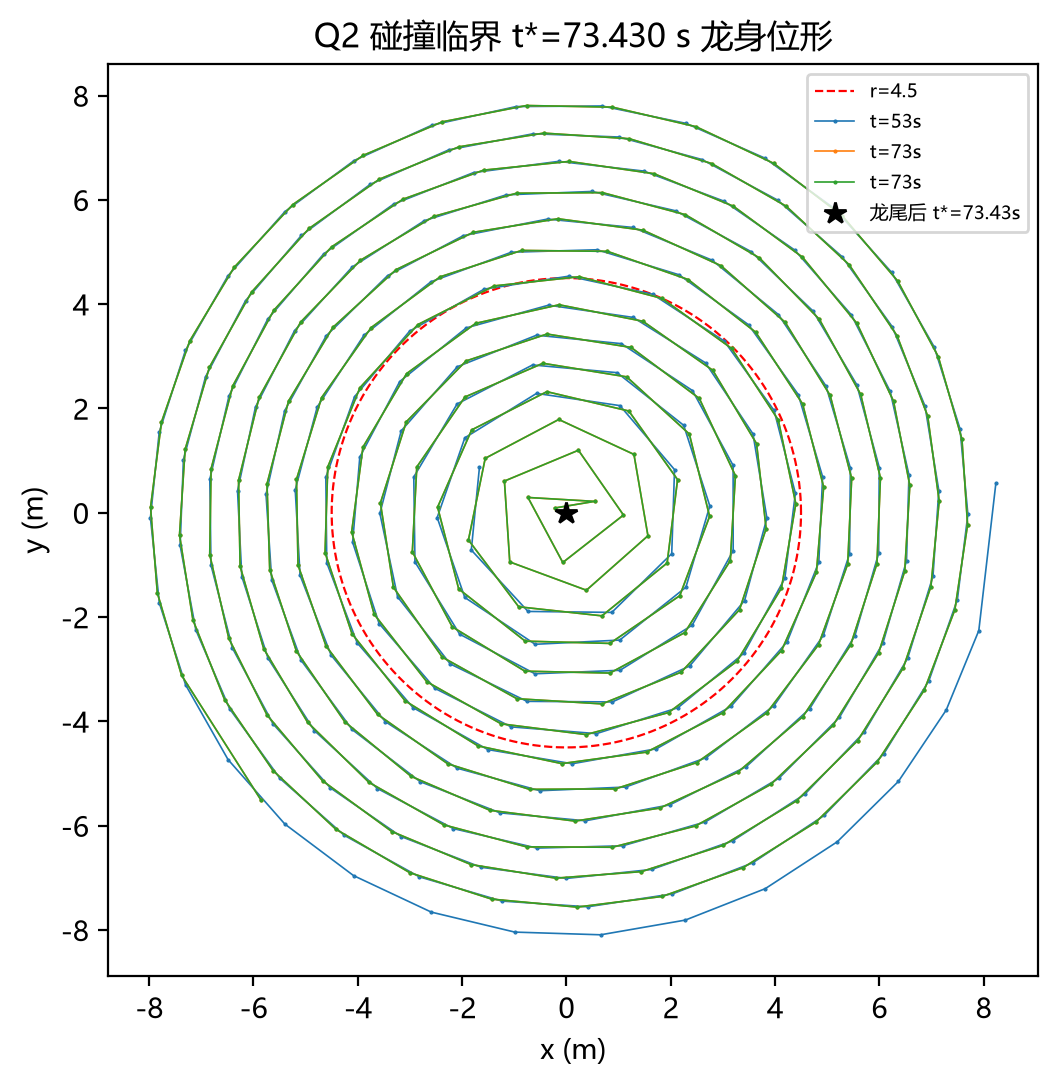
\includegraphics[width=0.78\textwidth]{../artifacts/figures/fig5_q2_collision.png}
\caption{问题二：$t^{\ast}$ 附近龙身位形（碰撞临界）[log:q2]}
\label{fig:q2}
\end{figure}

\subsection{结论与辩护}
由于链长（369.16m）远大于盘到 $r\to0$ 时可容纳的螺线弧长，盘入的物理极限由“尾部到达中心”决定，即 $t^{\ast}=73.43$s。此判据口径（尾越过中心 或 非相邻板段相交）已在论文假设与执行日志中明确；若评审关心对板段相交判据的依赖，第七章灵敏度提供两判据分别计算的对照。该口径与仲裁报告（$01a\_arbitration\_report.md$）一致。[log:q2]

\subsection{本章小结}
问题二给出盘入终止时刻 $t^{\ast}=73.4303$s（尾把手到达螺线中心），并交付终止时刻整队位置与速度。此结果是问题一在 $t>73.43$s 后龙尾位置钳制的物理来源，也是后续调头问题的前提条件。